\chapter{Cronograma}
\label{c.cronograma}

O projeto foi dividido nas seguintes etapas:

\begin{itemize}
    \item Estudo do tema;
    \item Elaboração do GDD;
    \item Elaboração do projeto de arquitetura;
    \item Estudo de modelos de IA;
    \item Escolha do modelo de IA e treinamento;
    \item Implementação do modelo de IA;
    \item Testes e adaptações necessárias;
    \item Desenvolvimento do jogo;
    \item Testes e revisões finais; e
    \item Redação da monografia.
\end{itemize}  

O momento de realização de cada uma dessas etapas é apresentado no Quadro \ref{cronograma}.\\


\begin{quadro}
    \centering
    \caption{Cronograma}
    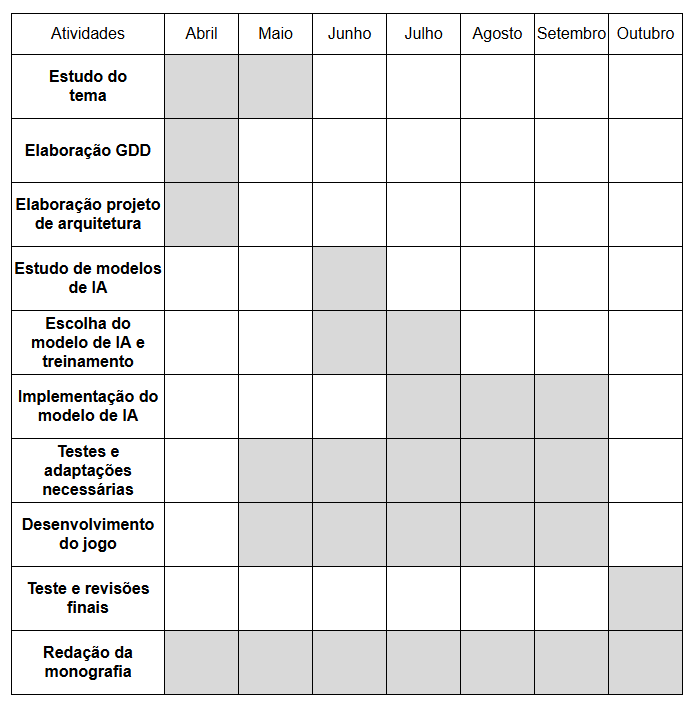
\includegraphics[width=1\linewidth]{figs/cronograma.PNG}
    \label{cronograma}
    \fonte{Elaborado pela autora.}
\end{quadro}


